\documentclass{UTNetLab}

\title{UDP and Its Applications}
\newcommand\reference{
   S. Panwar, S. Mao, J.-dong Ryoo, and Y. Li, “UDP and its applications,” in TCP/IP Essentials: A Lab-Based Approach, Cambridge: Cambridge University Press, 2004, pp. 100–110.
}

\begin{document}
	\section*{Objectives}
	\begin{itemize}
		\item Study \textbf{socket} as a traffic generator, in terms of its features and command line options.
		\item Study the User Datagram Protocol.
		\item IP fragmentation.
		\item MTU and path MTU discovery.
		\item UDP applications, using the Trivial File Transfer Protocol as an example.
		\item Compare UDP with TCP, using TFTP and the File Transfer Protocol (FTP).
	\end{itemize}
	
\part{Using the \texttt{socket} Program}
\label{sec:schema}
    In this lab, you will not need a router, only two hosts and one hub to connect the two hosts as shown in \hyperref[fig:5.0]{Figure~5.0} and \hyperref[tab:5.0]{Table~5.0}
    \begin{table}[H]
        \caption{Host IP addresses for \hyperref[fig:5.0]{Figure~5.0}}
        \label{tab:5.0}
        \centering
        \begin{tabular}{ *2c|*2c }
            \hline \hline
            \multicolumn{2}{c|}{Host\textsubscript{A}} & \multicolumn{2}{c}{Host\textsubscript{B}} \\
            Name & IP Address & Name & IP Address \\
            \hline 
            h0 & 128.238.61.100/24 & h1 & 128.238.61.101/24\\
            \hline \hline
            \end{tabular}
    \end{table}

    \begin{figure}[H]
        \centering
        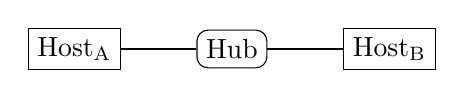
\begin{tikzpicture}
            \node[draw] (h1) at (-2,0){Host\textsubscript{A}};
            \node[draw,rounded corners] (hub) at (0,0){Hub};
            % \node[draw,rounded corners] (router) at (0,0){Router};
            % \node[draw,rounded corners] (hub1) at (2,0){Switch 1};
            \node[draw] (h0) at (2,0){Host\textsubscript{B}};
        
            \draw (h0) -- (hub) -- (h1);
        \end{tikzpicture}
        \caption{Simple router experiment (Figure~5.0)}        
        \label{fig:5.0}
    \end{figure}


\section{Socket Operation}
    Use the following commands in \textit{h0} and \textit{h1} as client and server hosts to observe the basic operation of \lstinline{socket}\footnote{Basic command is \lstinline{sock} use alternative \lstinline{socket} (rename of \lstinline{sock})} and \lstinline{echo} service.
    
     \fcolorbox{blue}{red!10}{{h\textsubscript{0}}'s Console}
    \lstset{backgroundcolor=\color{red!10}}
    \begin{lstlisting}
    socket -u 128.238.61.101 echo
    \end{lstlisting}
    
   \textbf{Note:} Type any text in socket and press Enter. Press \textit{CTRL+C} to exit.
   
   
    
     \fcolorbox{blue}{red!10}{{h\textsubscript{1}}'s Console}
    \lstset{backgroundcolor=\color{red!10}}
    \begin{lstlisting}
   	socket -s 5555 
    \end{lstlisting}
    
    \fcolorbox{blue}{red!10}{{h\textsubscript{0}}'s Console}
    \lstset{backgroundcolor=\color{red!10}}
    \begin{lstlisting}    	
    socket -i -n3 -w2048 128.238.61.101 5555
    \end{lstlisting}
    
    \textit{Note: }in general, this command is like \lstinline{socket} -i -n3 -w2048 \textit{server-host} 5555. 
     
    \begin{report}
    \item Explain the operation of each command.
    \end{report}

\section{\texttt{socket -h}}
    Study various options associated with the \lstinline{socket} program.
    A brief list of options can be displayed by typing \lstinline{socket}. More detailed discussion on socket can be found in Appendix~C of [5] in the reference book.
    
    \fcolorbox{blue}{red!10}{{h\textsubscript{0}}'s Console}
    \lstset{backgroundcolor=\color{red!10}}
    \begin{lstlisting}
    socket
    \end{lstlisting}

\section{Segment Size}
    While running \lstinline{wireshark} on \textit{your-host} or \textit{remote-host}, execute the following command with different values of size (i.e.\  the size of the datagram).
    
    \fcolorbox{blue}{lime!30}{{h\textsubscript{0}}'s Wireshark}
    \lstset{backgroundcolor=\color{lime!30}}
    \begin{lstlisting}
    Run wireshark on eth1

    \end{lstlisting}

    \fcolorbox{blue}{red!10}{{h\textsubscript{0}'s Console}}
   \lstset{backgroundcolor=\color{red!10}}
   \begin{lstlisting}
    socket -u -i -n1 -w100  128.238.61.101 echo
   \end{lstlisting}

 \textit{Note: }in general, this command is like \lstinline{socket} -u -i -n1 -w \textit{size} \textit{server-host} echo. 
    
    The \lstinline{-u} option is used to send UDP datagrams rather than TCP segments.

    Increase \textit{size} (i.e.\  the size of the datagram) until fragmentation occurs.

    Use \lstinline{netstat -in} to find out the MTU of the Ethernet interface.
    
    
    \fcolorbox{blue}{red!10}{{h\textsubscript{0}}'s Console}
    \lstset{backgroundcolor=\color{red!10}}
    \begin{lstlisting}
    netstat -in
    \end{lstlisting}
    \begin{report}
    \item What is the maximum value of \textit{size} for which the UDP datagram can be sent without IP fragmentation?
    Justify your answer with the \lstinline{netstat} output.
    \end{report}

\section{Datagram Fragmentation}
    Capture the data packets generated by the following command, while run \lstinline[emph={your-host, remote-host}]{tcpdump src host your-host} on \textit{h1}.
     
    \fcolorbox{blue}{red!10}{{h\textsubscript{1}}'s Console}
    \lstset{backgroundcolor=\color{red!10}}
    \begin{lstlisting}
     tcpdump -i eth1 src host 128.238.61.100
    \end{lstlisting}
    
    \fcolorbox{blue}{red!10}{{h\textsubscript{0}}'s Console}
    \lstset{backgroundcolor=\color{red!10}}
    \begin{lstlisting}
     socket -u -i -n1 -w10000 128.238.61.101  echo         
    \end{lstlisting}
    Save the \lstinline{tcpdump} output for the lab report.
    
    \begin{report}
    \item Explain the \lstinline{tcpdump} output in terms of the IP header fields that are used in fragmentation.

    \item When IP fragmentation occurs, only the first fragment has the UDP header.
    How do you verify this fact from the \lstinline{tcpdump} output?
    \end{report}


\section{Maximum Datagram Size}
\label{sec:MaxDatagramSize}
    While running \lstinline{wireshark}, execute the following command with different size values (for example 10000),
    
            \fcolorbox{blue}{lime!30}{{h\textsubscript{0}}'s Wireshark}
    \lstset{backgroundcolor=\color{lime!30}}
    \begin{lstlisting}
     Run wireshark on eth1
    \end{lstlisting}
    
        \fcolorbox{blue}{red!10}{{h\textsubscript{0}}'s Console}
    \lstset{backgroundcolor=\color{red!10}}
    \begin{lstlisting}
     socket -u -i -n1 -w10000 128.238.61.101 echo         
    \end{lstlisting}
 
    
    \textit{Note: }in general, this command is like \lstinline{socket} -u -i -n1 -w \textit{size} \textit{server-host} echo.
    
    in order to find out the maximum size of a UDP datagram that the system can send or receive, even when fragmentation is allowed.

    \begin{report}
    \item What is the maximum size of user data in a UDP datagram that the system can send or receive, even when fragmentation is allowed?
    \end{report}


\part{Path MTU Discovery Exercise}\label{sec:PMTUD}

\section{Discover path MTU}
    Connect the routers and the hosts as shown in \hyperref[fig:5.5]{Figure~5.5}. Change the IP addresses of all hosts accordingly (\textit{Note: }in Figure 5.5 that we've provided for you, these configurations are done).
    Note that the router IP addresses are the same as their default. Also you need to add route for all hosts to other subnets.
       
    \fcolorbox{blue}{red!10}{{h\textsubscript{0}}'s Console}
    \lstset{backgroundcolor=\color{red!10}}
    \begin{lstlisting}
    ip route add 128.238.62.0/24 dev eth1            
    \end{lstlisting} 

    
    \fcolorbox{blue}{red!10}{{h\textsubscript{1}}'s Console}
    \lstset{backgroundcolor=\color{red!10}}
    \begin{lstlisting}
    ip route add 128.238.61.0/24 dev eth1
    \end{lstlisting}

    % Open console of  each router, enable {RIP} routing (See Section~4.6 of reference book).

    Change the \texttt{MTU} of the \textit{ethernet1} interface of \textit{$R_{1}$} to 500 bytes (use \lstinline{enable} command first if needed).
    
\fcolorbox{blue}{yellow!10}{{R1\#}}
\lstset{backgroundcolor=\color{yellow!10}}
\begin{lstlisting}[frame=trBL,language={cisco}]
	config term
	R1(config)# int f1/0
	R1(config-if)# ip unreachables ! enables the router to send ICMP unreachable errors
	R1(config-if)# ip mtu 500
	! this command sets the IP layer MTU size
	! the real packet has 20 byte IP header (or more depending on the options value)
	R1(config-if)# mtu 500 ! may not be supported (can see: mtu ?)
	! this command sets the ethernet layer MTU size

\end{lstlisting}

\textit{Note: }the sentences written after \textbf{!} are comments and do not need to be run. 
   
    Test connectivity by \lstinline{ping}ing the hosts in the other subnets. After you can reach the hosts in the other subnets, run \lstinline{wireshark} on your host.
    
   \fcolorbox{blue}{red!10}{{h\textsubscript{0}}'s Console}
   \lstset{backgroundcolor=\color{red!10}}
   \begin{lstlisting}[frame=trBL,language={cisco}]
 	ping 128.238.62.101 
 	! After you reach the hosts in the other subnets, press Ctrl+Z to stop the ping command.
   \end{lstlisting} 
   
   \fcolorbox{blue}{lime!30}{{h\textsubscript{0}}'s Wireshark}
   \lstset{backgroundcolor=\color{lime!30}}
  \begin{lstlisting}
    Run wireshark on eth1
  \end{lstlisting} 
  
    Start a UDP socket server on \textit{remote-host}, using \lstinline{socket -u -s 5555} on \textit{h1}.   
    
     \fcolorbox{blue}{red!10}{{h\textsubscript{1}}'s Console}
    \lstset{backgroundcolor=\color{red!10}}
    \begin{lstlisting}
    socket -u -s 5555
    \end{lstlisting}

 Then run the socket client from \textit{h0}:
    
    \fcolorbox{blue}{red!10}{{h\textsubscript{0}}'s Console}
  \lstset{backgroundcolor=\color{red!10}}
  \begin{lstlisting}
   	socket -i -u  -n10 -w1200 -p5  128.238.62.101  5555
  \end{lstlisting}

    \begin{table}[H]
        \caption{Router and Host IP addresses for \hyperref[fig:5.5]{Figure~5.5} (Table~5.5)}
        \centering
        \begin{tabular}{ *2c|*2c|*2c }
            \hline \hline
            \multicolumn{2}{c|}{Router} & \multicolumn{2}{c|}{Host\textsubscript{A}} & \multicolumn{2}{c}{Host\textsubscript{B}} \\
            f0/0 & f1/0 & Name & IP Address & Name & IP Address \\
            \hline 
            128.238.61.1/24 & 128.238.62.1/24 & h0 & 128.238.61.101/24 & h1 & 128.238.62.101/24 \\
            \hline \hline
            \end{tabular}
    \end{table}

    \begin{figure}[H]
        \centering
        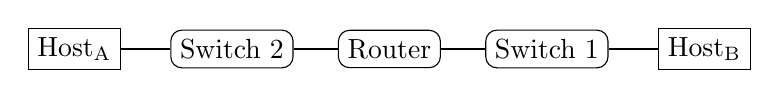
\begin{tikzpicture}
            \node[draw] (h1) at (-4,0){Host\textsubscript{A}};
            \node[draw,rounded corners] (hub2) at (-2,0){Switch 2};
            \node[draw,rounded corners] (router) at (0,0){Router};
            \node[draw,rounded corners] (hub1) at (2,0){Switch 1};
            \node[draw] (h0) at (4,0){Host\textsubscript{B}};
        
            \draw (h0) -- (hub1);
            \draw (h1) -- (hub2);
            \draw[thick] (hub1) -- (router);
            \draw[thick] (hub2) -- (router);
        \end{tikzpicture}
        \caption{The network setup for \nameref{sec:PMTUD} (Figure~5.5/Figure~4.10)}
        \label{fig:5.5}
    \end{figure}


    Observe the DF bit of the first datagram and that of the following datagrams. Save the \lstinline{wireshark} output for your lab report.

    \begin{report}
    \item Explain the operation of path MTU discovery based on the \lstinline{wireshark} outputs saved.
    
    \item Which ICMP message is used in path MTU discovery? Give the decimal value of each field of the captured ICMP message.
    
    \item What is the MTU of the destination network of the UDP datagram? Verify your answer using both the ICMP message and the IP fragmentation trace saved.
    \end{report}

\part{Exercises with FTP and TFTP}
    Use first network (section \nameref{sec:schema}) topology (Figure 5.0) for this exercise.
    We will study the performance of FTP and TFTP for file transfer between two machines.
    By transferring the same file using these two protocols, we can compare the operations and performances of UDP and TCP. 

    Four files (\path{large.dum}, \path{med.dum}, \path{small.dum} and \path{thin.dum}) with random contents are stored in the \path{/home/netlab}\footnote{We change original path (\path{/tftpboot}) to \path{/home/netlab} to be same as ftp user path.} directory of each host in the lab.
    We will use the \lstinline{get} command to retrieve files from a remote host.
    When FTP is used, you need to change the directory to \path{/home/netlab/} by using \lstinline{cd /home/netlab} before retrieving the file.
    If you don’t know how to use \lstinline{tftp}, refer to its manual page.
    
    \section{TFTP and FTP}
    In order to compare the transfer rates of FTP and TFTP, we will retrieve all large, med, small and thin files from a remote server using FTP and TFTP, respectively.

    First run  \lstinline{wireshark} on host \textit{h0}:
    
    \fcolorbox{blue}{lime!30}{{h\textsubscript{0}}'s Wireshark}
    \lstset{backgroundcolor=\color{lime!30}}
    \begin{lstlisting}
    Run wireshark on eth1, Filter: ip.addr == 128.238.61.100 && ip.addr == 128.238.61.101
       
    \end{lstlisting}

    %\textit{Note: }You can use the redirect operator, \lstinline{>}, to save the \lstinline{tcpdump} output into a text file for large \lstinline{tcpdump} outputs and read it with \lstinline{less, grep, nano} or \lstinline{vim}.
    %For example you can change previous command into:
    
      %\fcolorbox{blue}{Green!10}{{h\textsubscript{0}}'s Console}
   %\lstset{backgroundcolor=\color{green!10}}
   %\begin{lstlisting}
   %tcpdump host 128.238.61.100 and 128.238.61.101 > output.dump      
   %end{lstlisting}
    
    Now you should repeat this scenario for all files (\path{large.dum}, \path{med.dum}, \path{small.dum} and \path{thin.dum}).
    
      \fcolorbox{blue}{green!10}{{h\textsubscript{0}'s Console}}
    \lstset{backgroundcolor=\color{green!10}}
    \begin{lstlisting}[frame=trBL,language={cisco}]
    $ ls /etc/xinetd.d/		 ! see services in xinetd
    $ tftp host
    tftp> get $filename		 ! thin, small, med, large
    tftp> quit
    $ ftp host 				 ! Enter user and password -> netlab and netlab
    ftp> ls
    ftp> get $filename		 ! thin, small, med, large
    ftp> quit
    
    \end{lstlisting}
    
    \textit{Note: }For example, we run below commands for file \textit{small.dum}. \underline{You should repeat these commands for other files.}
    
    \fcolorbox{blue}{red!10}{{h\textsubscript{0}'s Console}}
    \lstset{backgroundcolor=\color{red!10}}
    \begin{lstlisting}
    ls /etc/xinetd.d/
    tftp 128.238.61.101
    tftp> get small.dum
    tftp> quit
    ftp 128.238.61.101  # Enter user and password -> netlab and netlab
    ftp> ls
    ftp> get small.dum
    ftp> quit  
    \end{lstlisting}
   
    % Create \path{small.dum} with 10kB, \path{med.dum} with 1MB and \path{larg.dum} with 50MB.

    Also, from the \lstinline{ftp} window, record the transfer rate (time) displayed. 
  
    \begin{report}
    \item Examining the saved \lstinline{wireshark} output. Identify the starting and ending time of actual data transfer.
    Don’t include the time spent establishing the TCP connection.
    Calculate the time spent for data transfer. 

    \item Compare the time with the value displayed in \lstinline{ftp} window.
    Are they consistent?
    If there exists any significant difference, what might be the reason? 

    \item Now, from the second session, carefully determine the starting and ending time of data transfer for the \lstinline{tftp} program. 

    \item Compare the time with the value displayed in \lstinline{tftp} window.
    Are they consistent?
    If there exists any significant difference, what might be the reason? 

    \item By comparing the actual data transfer times of \lstinline{ftp} and \lstinline{tftp}, which of these two is faster, and why?
    \end{report}

\section{TFTP Analysis}
    Capture the packets that are exchanged during a \lstinline{tftp} session for the \path{/home/netlab/small.dum} file between \textit{h0} and \textit{h1}, using:
    
    \fcolorbox{blue}{lime!30}{{h\textsubscript{0}}'s Wireshark}
    \lstset{backgroundcolor=\color{lime!30}}
    \begin{lstlisting}
    Run wireshark on eth1, Filter: ip.addr == 128.238.61.100 && ip.addr == 128.238.61.101
     
    \end{lstlisting}
    
    \fcolorbox{blue}{red!10}{{h\textsubscript{0}'s Console}}
    \lstset{backgroundcolor=\color{red!10}}
    \begin{lstlisting}
    tftp 128.238.61.101
    tftp> get small.dum
    tftp> quit
    \end{lstlisting}
    Observe the protocol in action.    Analyze various types of TFTP messages. Save \lstinline{wireshark} output for the lab report.
    
    \begin{report}
        \item List all the different types of packets exchanged during the \lstinline{tftp} session. Compare them with the TFTP message format in \hyperref[fig:5.3]{Figure~5.3} of reference book.

        Why does the server’s port number change?
        
        \item In most cases, \lstinline{tftp} service is restricted.\footnote{This is not the case in our lab, where we deliberately enabled the \lstinline{tftp} service and use it as a tool to study the UDP protocol.}
        Why is \lstinline{tftp} service not generally available to users? At least write two problem of \lstinline{tftp} protocol.
        
        \item In \autoref{sec:MaxDatagramSize}, we found the maximum size of a UDP datagram in your machine. With \lstinline{tftp}, which uses UDP, we transferred a file larger than the maximum UDP datagram size.
        How do you explain this?
    \end{report}

\section{FTP Small File}
    Repeat the above experiment, but use \lstinline{ftp}.
    Capture a trace of the packets exchanged when downloading the \path{/home/netlab/small.dum} file using \lstinline{ftp}.

    Examine the port numbers used.
    
        \fcolorbox{blue}{lime!30}{{h\textsubscript{0}}'s Console}
    \lstset{backgroundcolor=\color{lime!30}}
    \begin{lstlisting}
    Run wireshark on eth1, Filter: ip.addr == 128.238.61.100 && ip.addr == 128.238.61.101
      
    \end{lstlisting}
    
    \fcolorbox{blue}{red!10}{{h\textsubscript{0}'s Console}}
    \lstset{backgroundcolor=\color{red!10}}
    \begin{lstlisting}
    ftp 128.238.61.101		# Enter user and password -> netlab and netlab
    ftp> get small.dum
    ftp> quit
    \end{lstlisting}
    
    
    \begin{report}
        \item How many well-known port numbers were used?
        Which machine used the well-known port numbers?
        What were the other machine’s port numbers?
        
        \item As can be seen from the \lstinline{wireshark} output, FTP involves two different connections, \texttt{ftp-control} and \texttt{ftp-data}.
        Why are two different connections used, instead of one connection?
    \end{report}

\section{FTP Debug}
    Run \lstinline{ftp} in \textit{your-host} using the debug mode: \lstinline[emph={your-host, remote-host}]{ftp -d remote-host}.
    
     \fcolorbox{blue}{red!10}{{h\textsubscript{0}}'s Console}
    \lstset{backgroundcolor=\color{red!10}}
    \begin{lstlisting}
    ftp -d 128.238.61.101  		 # Enter user and password -> netlab and netlab    
    \end{lstlisting}
    After logging into the remote host, type \lstinline{dir /home/netlab/small.dum} in the \lstinline{ftp} window.
    
    \fcolorbox{blue}{red!10}{{h\textsubscript{0}}'s Console}
    \lstset{backgroundcolor=\color{red!10}}
    \begin{lstlisting}
    ftp> dir /home/netlab/small.dum    
    \end{lstlisting}
    Then type \lstinline{quit} to terminate the \lstinline{ftp} session, and save the \lstinline{ftp} window output.
    
    \fcolorbox{blue}{red!10}{{h\textsubscript{0}}'s Console}
    \lstset{backgroundcolor=\color{red!10}}
    \begin{lstlisting}
    ftp> quit    
    \end{lstlisting}
    \begin{report}
    \item Submit what you saved in this exercise, explaining each line of the output.
    Explain how the \lstinline{PORT} command works.
    Which connection, the control connection or the data connection, did the server send the response (the \lstinline{LIST} output) on?
    \end{report}

\end{document}